\documentclass{article}
\usepackage{tikz}
\usepackage{amsmath, amssymb}

\newcommand{\warningbox}[2]{%
\vspace{0.25em}%
\noindent\begin{tikzpicture}%
\node[draw=orange, line width=1.4pt, fill=orange!8, rounded corners=4pt, inner sep=6pt, text width=8cm] {%
  \textbf{Warning: #1}\[0.15em]%
  {\small #2}%
};%
\end{tikzpicture}%
\vspace{0.25em}%
}

\begin{document}
  \begin{itemize}
    \item \textbf{Question Answered?} Yes, with a clear decision rule: drive at legal limit {\max} = 110\text{ km/h}$ whenever $\mu > \mu^*$ ( > 6.27\text{ EUR/h}$); otherwise cruise at ^* = [(b+\mu d)/(2c)]^{1/3}$.
    \item \textbf{Hypotheses Evaluated:}
      \begin{itemize}
        \item \textbf{H1 Supported:} Minimizing energy alone yields  \approx 42\text{ km/h}$, which is dangerously slow and legally prohibited on motorways.
        \item \textbf{H2 Supported:} Realistic commercial wages (5\text{--}25\text{ EUR/h} > 6.3\text{ EUR/h}$) place operations firmly on the {\max}$ boundary plateau.
        \item \textbf{H3 Supported:} Interior optimum exists only for low time-value ($\mu < \mu^*$). Flat curvature ( c_E c \delta^2$) renders costs highly forgiving to small speed deviations ($\pm 5\text{ km/h} \implies < 0.1\%$ cost increase).
        \item \textbf{H4 Refuted:} Route length $ scales both energy and time terms proportionally, making ^*$ independent of $. Route length matters solely when delivery deadlines ((v) \le T_{\max}$) bind.
      \end{itemize}
    \item \textbf{Limiting Cases \& Convexity:} $\lim_{\mu \to 0} v^* = v_E$. Second derivative ''(v^*) = 6 c_E c > 0$ strictly guarantees global optimality and uniqueness.
    \item \textbf{Sensitivity:} $ increased by $+20\%$ shifts ^*$ down by only hBc5.9\%$ (factor .2^{-1/3}$). Time cost  +20\%$ shifts ^*$ by at most $+6.3\%$.
    \item \textbf{Limitations:} Unpriced battery degradation and safety risk (handled indirectly via {\max}$), constant gradient, no traffic waves or charging stops.
    \item \textbf{Additional Data Needed:} Fleet telematics for calibrated ,b,c$, empirical late-delivery penalties, real vehicle depreciation curves.
  \end{itemize}

  \warningbox{Optimal speed $\neq$ Fastest speed $\neq$ Most energy-efficient speed.}{True cost optimality balances energy expenditure against productive labor utility.}
  
  \warningbox{Better fit $\neq$ Better model.}{High-degree regression without aeromechanical basis produces unphysical non-convexities.}

  \vspace{0.2em}
  % Closing Lecture Strip
  \centering
  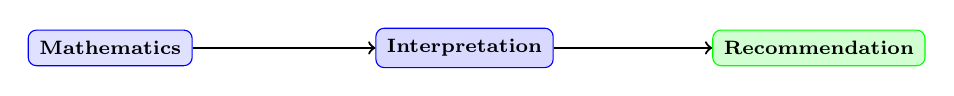
\begin{tikzpicture}
    \node[draw=blue, fill=blue!12, rounded corners=3pt, font=\scriptsize\bfseries, inner sep=4pt] (m) at (0,0) {Mathematics};
    \node[draw=blue, fill=blue!15, rounded corners=3pt, font=\scriptsize\bfseries, inner sep=4pt] (i) at (4.5,0) {Interpretation};
    \node[draw=green, fill=green!18, rounded corners=3pt, font=\scriptsize\bfseries, inner sep=4pt] (r) at (9.0,0) {Recommendation};
    \draw[->, thick] (m) -- (i);
    \draw[->, thick] (i) -- (r);
  \end{tikzpicture}
\end{document}
